\documentclass[11pt,a4paper]{article}
\usepackage[margin=2.5cm]{geometry}
\usepackage{amsmath,amssymb}
\usepackage{graphicx}
\usepackage[hidelinks]{hyperref}
\usepackage{parskip}
\usepackage{booktabs}
\usepackage[UKenglish]{babel}

\title{S2 Major Module Coursework\\Written Answers}
\author{Rowan D'Auria}
\date{Lent Term 2026}

\begin{document}
\maketitle

%----------------------------------------------------------------------
\section*{Question 1 --- Accident data}
%----------------------------------------------------------------------

The mean rate of accidents over the full observation period is
\[
\bar{x} = \frac{N}{L} = \frac{191}{40550} \approx 4.710 \times 10^{-3} \;\text{accidents per day.}
\]

\begin{figure}[ht]
  \centering
  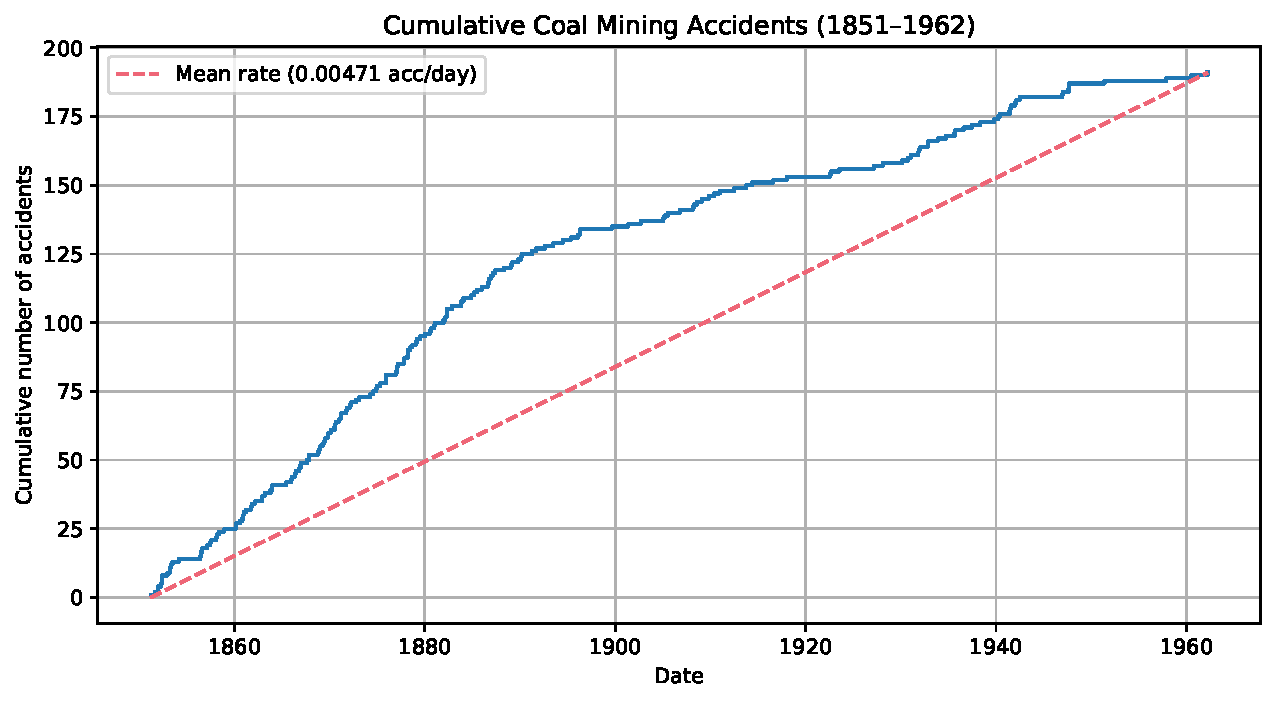
\includegraphics[width=0.85\textwidth]{figs/q1_cumulative_accidents.pdf}
  \caption{Cumulative number of mining accidents (1851--1962). The dashed line shows the overall mean rate.}
  \label{fig:q1}
\end{figure}

%----------------------------------------------------------------------
\section*{Question 2 --- Priors}
%----------------------------------------------------------------------

\subsection*{(a) Comparing change-point priors}

The plain order statistics prior draws $k$ uniform points on $[0, L]$ and sorts them.
The even-numbered order statistics prior instead draws $2k + 1$ uniform points and retains every second one (the even-numbered order statistics).
Because each retained change point has an ``escort'' point on either side, the even-numbered order statistics prior discourages change points from clustering together or from sitting near the boundaries.
In effect, the escort points act as spacers: a gap $g_j$ between adjacent change points enters the density as a factor of $g_j$, penalising small gaps.

Figure~\ref{fig:q2a} illustrates this for $k = 4$.
The marginal distributions of individual change points are more peaked and pushed away from the endpoints under the even-numbered prior.
The plain order statistics prior, by contrast, allows change points to cluster more freely and to approach $0$ or $L$.
The even-numbered prior therefore favours configurations where change points are more evenly spread across the observation window, which is a sensible default when there is no prior reason to expect clustering.

\begin{figure}[ht]
  \centering
  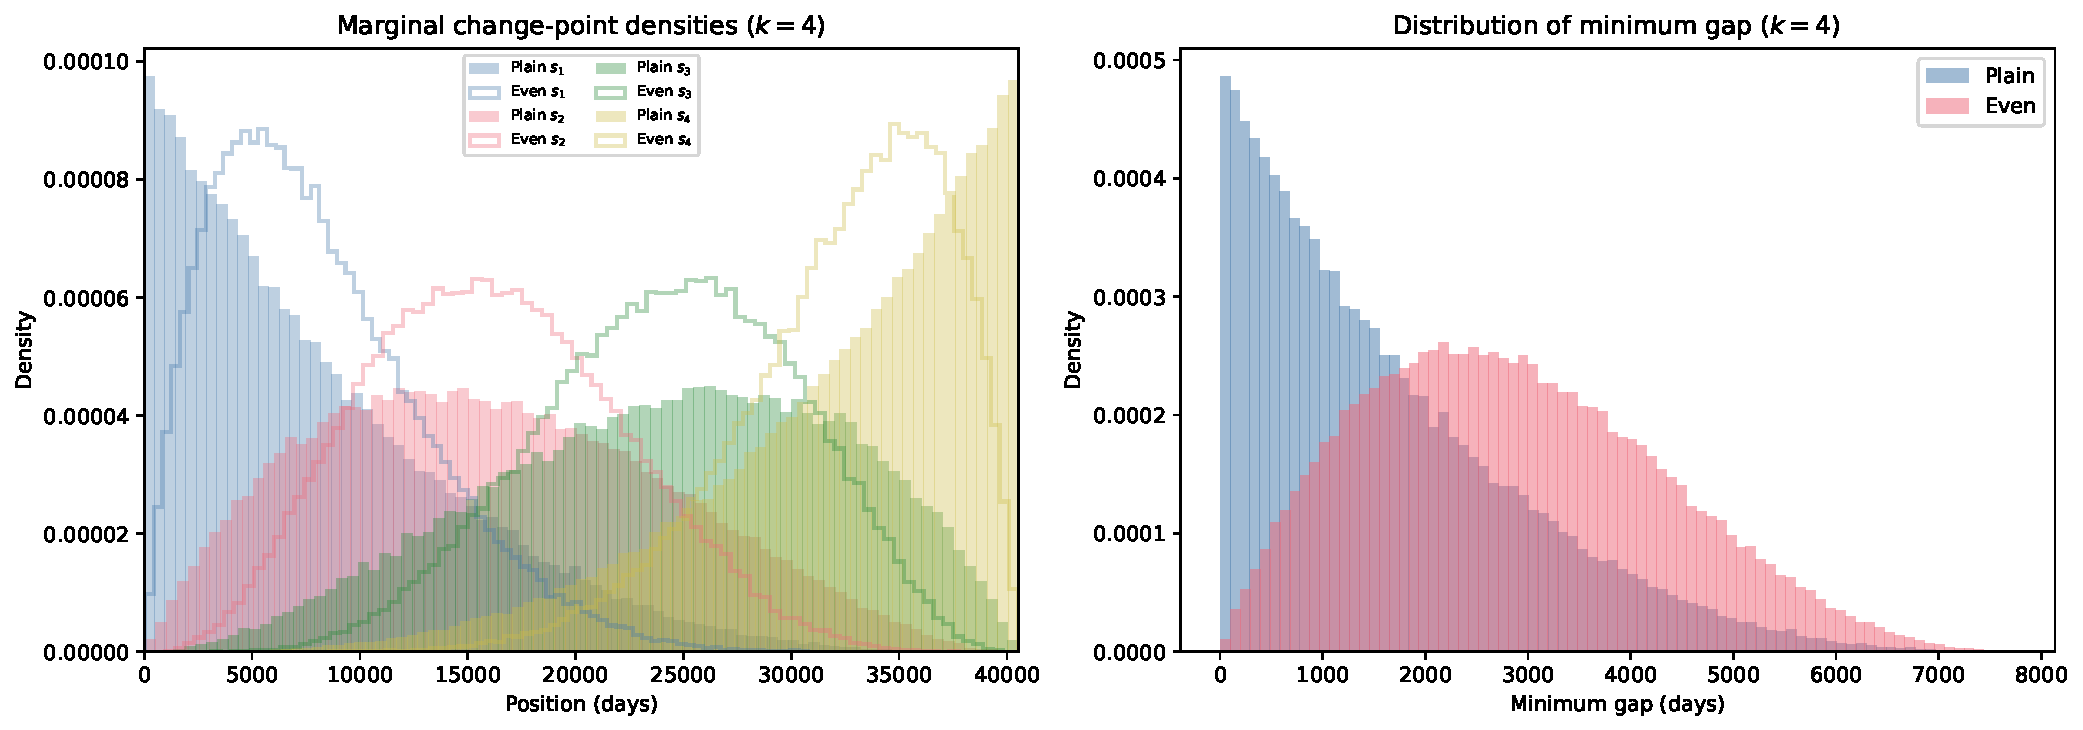
\includegraphics[width=\textwidth]{figs/q2a_changepoint_priors.pdf}
  \caption{Marginal distributions of individual change points for $k=4$ under the plain order statistics prior (left) and even-numbered order statistics prior (right).}
  \label{fig:q2a}
\end{figure}

\subsection*{(b) Derivation of the even-numbered order statistics prior}

The PDF of the plain order statistics of $2k+1$ uniform random variables on $[0,1]$ is
\[
  P(u_{(1)}, u_{(2)}, \ldots, u_{(2k+1)}) = (2k+1)!
\]
on the region $0 < u_{(1)} < u_{(2)} < \cdots < u_{(2k+1)} < 1$.

The even-numbered order statistics are $\hat{s}_j = u_{(2j)}$ for $j = 1, \ldots, k$.
To obtain their marginal density, we integrate out the $k+1$ odd-indexed variables $u_{(1)}, u_{(3)}, \ldots, u_{(2k+1)}$.

Each odd variable $u_{(2j-1)}$ is constrained to the interval $[\hat{s}_{j-1},\, \hat{s}_j]$ (using the conventions $\hat{s}_0 = 0$, $\hat{s}_{k+1} = 1$). Since the integrand is constant in each odd variable, each integral contributes a factor equal to the length of its support:
\[
  \int_{\hat{s}_{j-1}}^{\hat{s}_j} \mathrm{d}u_{(2j-1)} = \hat{s}_j - \hat{s}_{j-1} = \hat{g}_j.
\]

Performing all $k + 1$ such integrals (for $u_{(1)}, u_{(3)}, \ldots, u_{(2k+1)}$) gives
\[
  P(\hat{s}_1, \hat{s}_2, \ldots, \hat{s}_k) = (2k+1)!\,\prod_{j=1}^{k+1} \hat{g}_j \;\propto\; \prod_{j=1}^{k+1} \hat{g}_j\,,
\]
where $\hat{g}_j = \hat{s}_j - \hat{s}_{j-1}$ are the gaps on the unit interval.

Rescaling to the observation interval via $s_j = L\hat{s}_j$ gives $g_j = L\hat{g}_j$, so
\[
  \boxed{\pi(s_1, s_2, \ldots, s_k \mid M_k) \;\propto\; \prod_{j=1}^{k+1} g_j\,.}
\]

%----------------------------------------------------------------------
\section*{Question 3 --- The constant rate model, $M_0$}
%----------------------------------------------------------------------

\subsection*{(a) Prior and posterior for $h_0$; evidence $Z_0$}

Under $M_0$ the rate is constant at $h_0$ with prior $h_0 \sim \Gamma(1, 200)$, i.e.\ $\pi(h_0) = 200\,e^{-200 h_0}$.
The likelihood is $\mathcal{L} = h_0^N e^{-h_0 L}$, so the unnormalised posterior is $h_0^N e^{-h_0(L + \beta)}$, which is a Gamma distribution with shape $\alpha + N = 192$ and rate $\beta + L = 40750$.

Figure~\ref{fig:q3a} compares the prior and posterior.
The prior is an exponential distribution broadly spread over small rates, while the posterior is sharply concentrated around $h_0 \approx N/(L + \beta) \approx 4.71 \times 10^{-3}$ accidents per day --- essentially the observed mean rate.
The data are highly informative: the posterior is orders of magnitude narrower than the prior.

The evidence is computed analytically:
\[
  Z_0 = \int_0^\infty \pi(h_0)\,\mathcal{L}(\{I_i\} \mid h_0)\,\mathrm{d}h_0
       = \frac{\beta^\alpha\,\Gamma(\alpha + N)}{(\beta + L)^{\alpha + N}}
       \implies \log Z_0 = -1217.09.
\]
This was verified by numerical integration, yielding identical results.

\begin{figure}[ht]
  \centering
  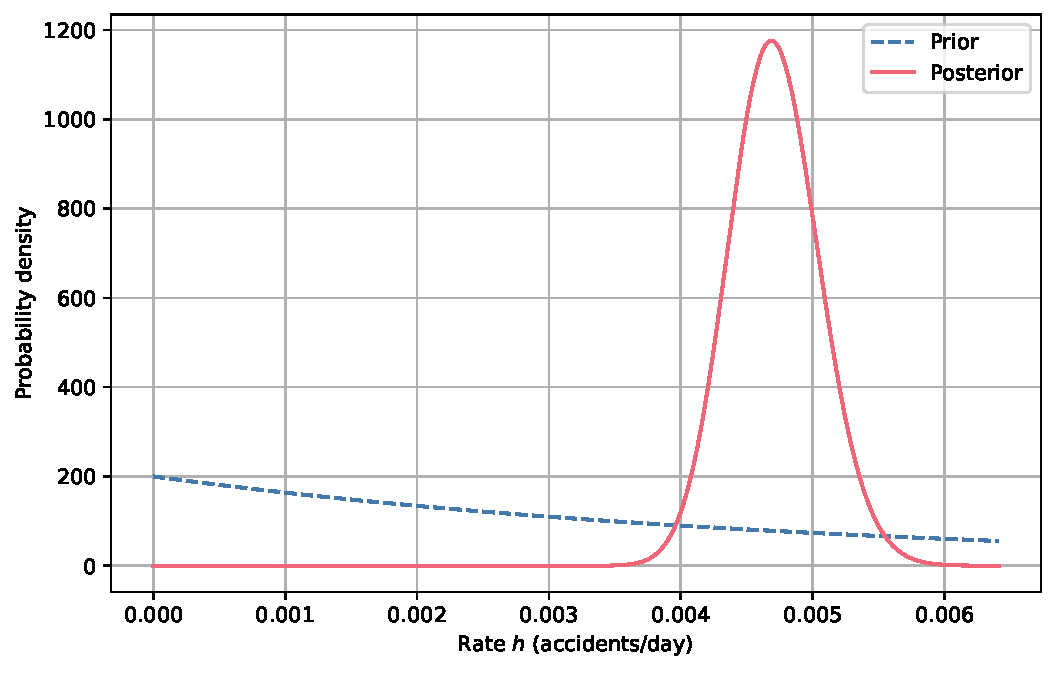
\includegraphics[width=0.7\textwidth]{figs/q3a_m0_prior_posterior.pdf}
  \caption{Prior and normalised posterior for the constant accident rate $h_0$ under model $M_0$.}
  \label{fig:q3a}
\end{figure}

%----------------------------------------------------------------------
\section*{Question 4 --- The 1 change-point model, $M_1$}
%----------------------------------------------------------------------

\subsection*{(a) MCMC posterior sampling}

We sampled the $M_1$ posterior using \texttt{emcee} (Foreman-Mackey et al., 2013), an affine-invariant ensemble sampler.
Unlike gradient-based methods (e.g.\ NUTS), \texttt{emcee} requires only pointwise evaluation of the log-posterior, which suits the piecewise-constant likelihood that is non-differentiable at $s_1$.
We used 32 walkers initialised in a tight ball around a reasonable starting point ($h_0 \approx 0.009$, $h_1 \approx 0.003$, $s_1 \approx 14\,000$ days).
After a burn-in of 2000 steps the sampler was reset and run for a further 10\,000 production steps.

The priors are $h_0, h_1 \sim \Gamma(1, 200)$ and $s_1/L \sim \text{Beta}(2, 2)$ (the even-numbered order statistics prior for $k = 1$).

Convergence was assessed via: (i) visual inspection of trace plots (Figure~\ref{fig:q4a_trace}, showing good mixing with no trends); (ii) integrated autocorrelation times ($\tau_{h_0} \approx 49$, $\tau_{h_1} \approx 49$, $\tau_{s_1} \approx 48$ steps), yielding roughly 6500 effective samples; and (iii) the mean acceptance fraction of $0.52$, within the recommended range for \texttt{emcee}.

The posterior medians and 68\% credible intervals are $h_0 = 0.0086 \pm 0.0008$, $h_1 = 0.0025 \pm 0.0003$, and $s_1 = 14\,362 \pm 770$ days (corresponding to $\sim$1890).
The corner plot (Figure~\ref{fig:q4a_corner}) shows a clear separation between $h_0$ and $h_1$, confirming that the data strongly favour a decrease in accident rate.

\begin{figure}[ht]
  \centering
  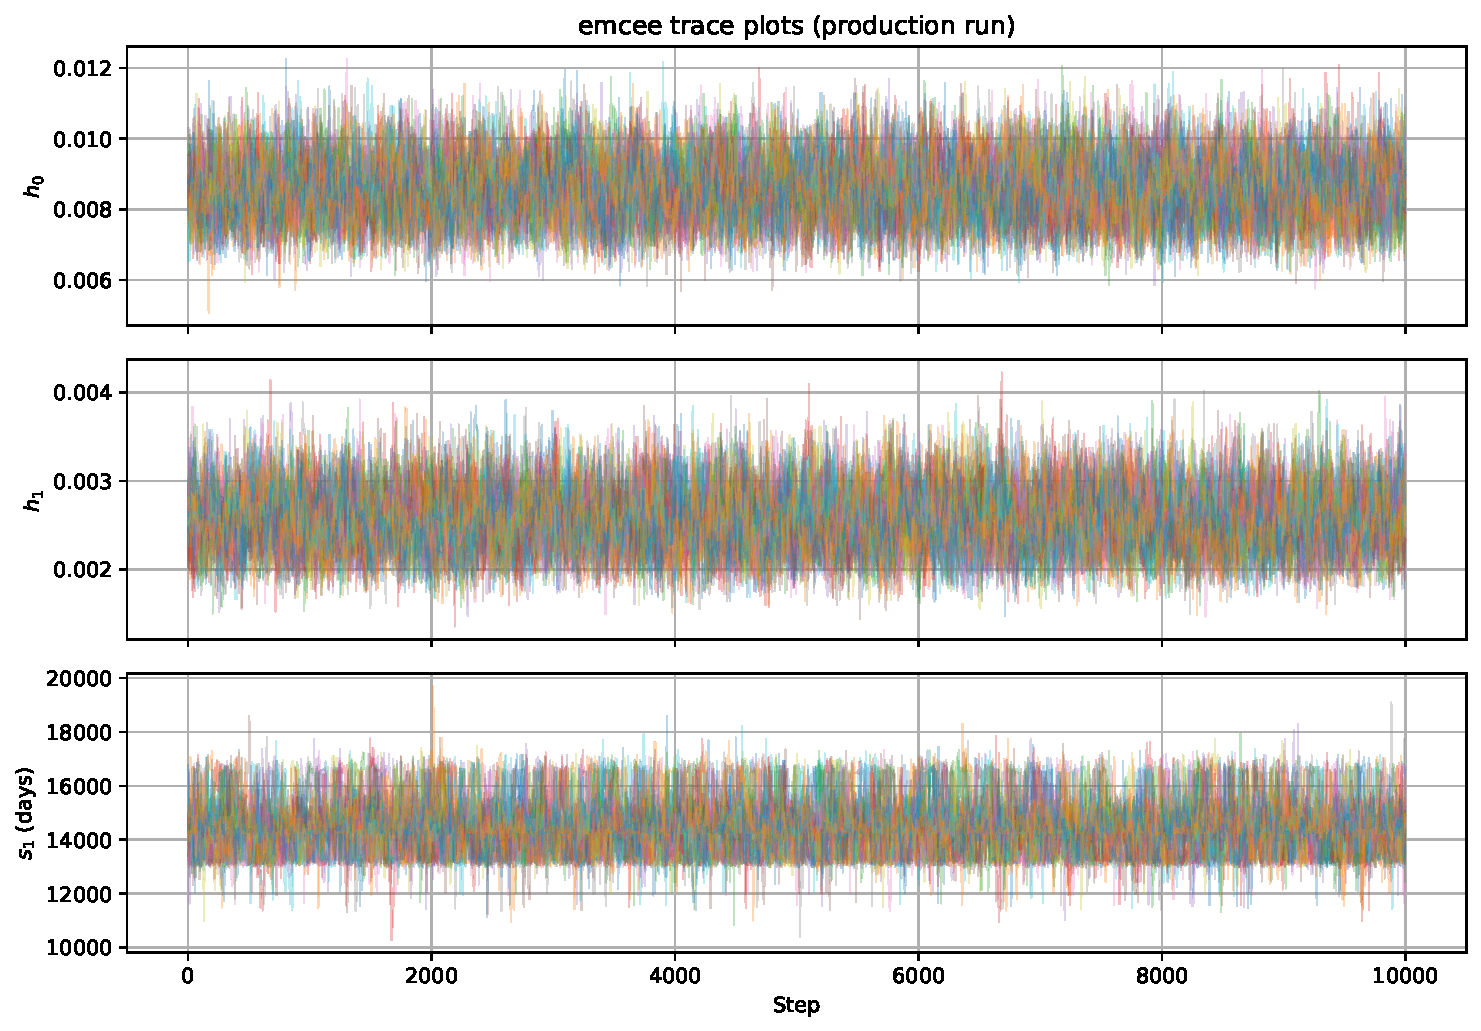
\includegraphics[width=0.85\textwidth]{figs/q4a_m1_trace_plots.pdf}
  \caption{Trace plots for the $M_1$ parameters from the \texttt{emcee} production run.}
  \label{fig:q4a_trace}
\end{figure}

\begin{figure}[ht]
  \centering
  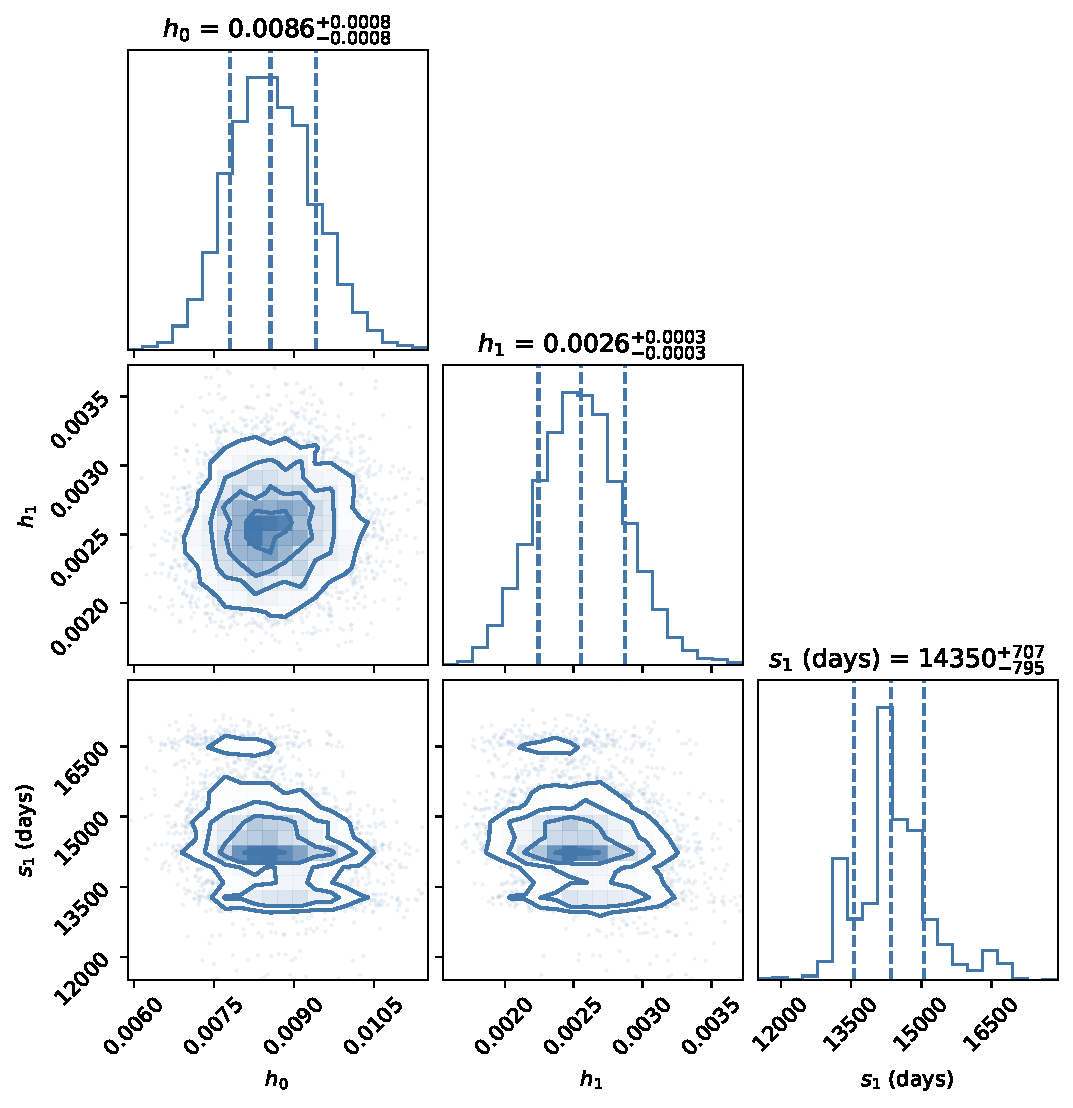
\includegraphics[width=0.7\textwidth]{figs/q4a_m1_corner.pdf}
  \caption{Corner plot for the $M_1$ posterior.}
  \label{fig:q4a_corner}
\end{figure}

\subsection*{(b) Savage--Dickey density ratio}

The Savage--Dickey density ratio provides the Bayes factor between nested models without computing evidences explicitly.
Model $M_0$ is recovered from $M_1$ by setting $h_0 = h_1$ (equivalently $\delta = h_0 - h_1 = 0$).
The Bayes factor is then
\[
  B_{01} = \frac{Z_0}{Z_1} = \frac{p(\delta = 0 \mid \{I_i\}, M_1)}{\pi(\delta = 0 \mid M_1)},
\]
i.e.\ the ratio of the posterior to prior density of $\delta$ evaluated at $\delta = 0$.

The difficulty is twofold.
First, the unconstrained $M_1$ posterior concentrates around $\delta \approx 0.006$, far from zero --- the data strongly favour distinct rates.
No MCMC samples visit $\delta \approx 0$, so any kernel density estimate of the posterior at that point is unreliable.
Second, when we enforce $h_0 = h_1$ the change point $s_1$ becomes completely unidentifiable: with equal rates on both sides, $s_1$ has no effect on the likelihood and simply follows its prior (Figure~\ref{fig:q4b}).
This degeneracy at the nested point means the Savage--Dickey ratio cannot be practically evaluated.

\begin{figure}[ht]
  \centering
  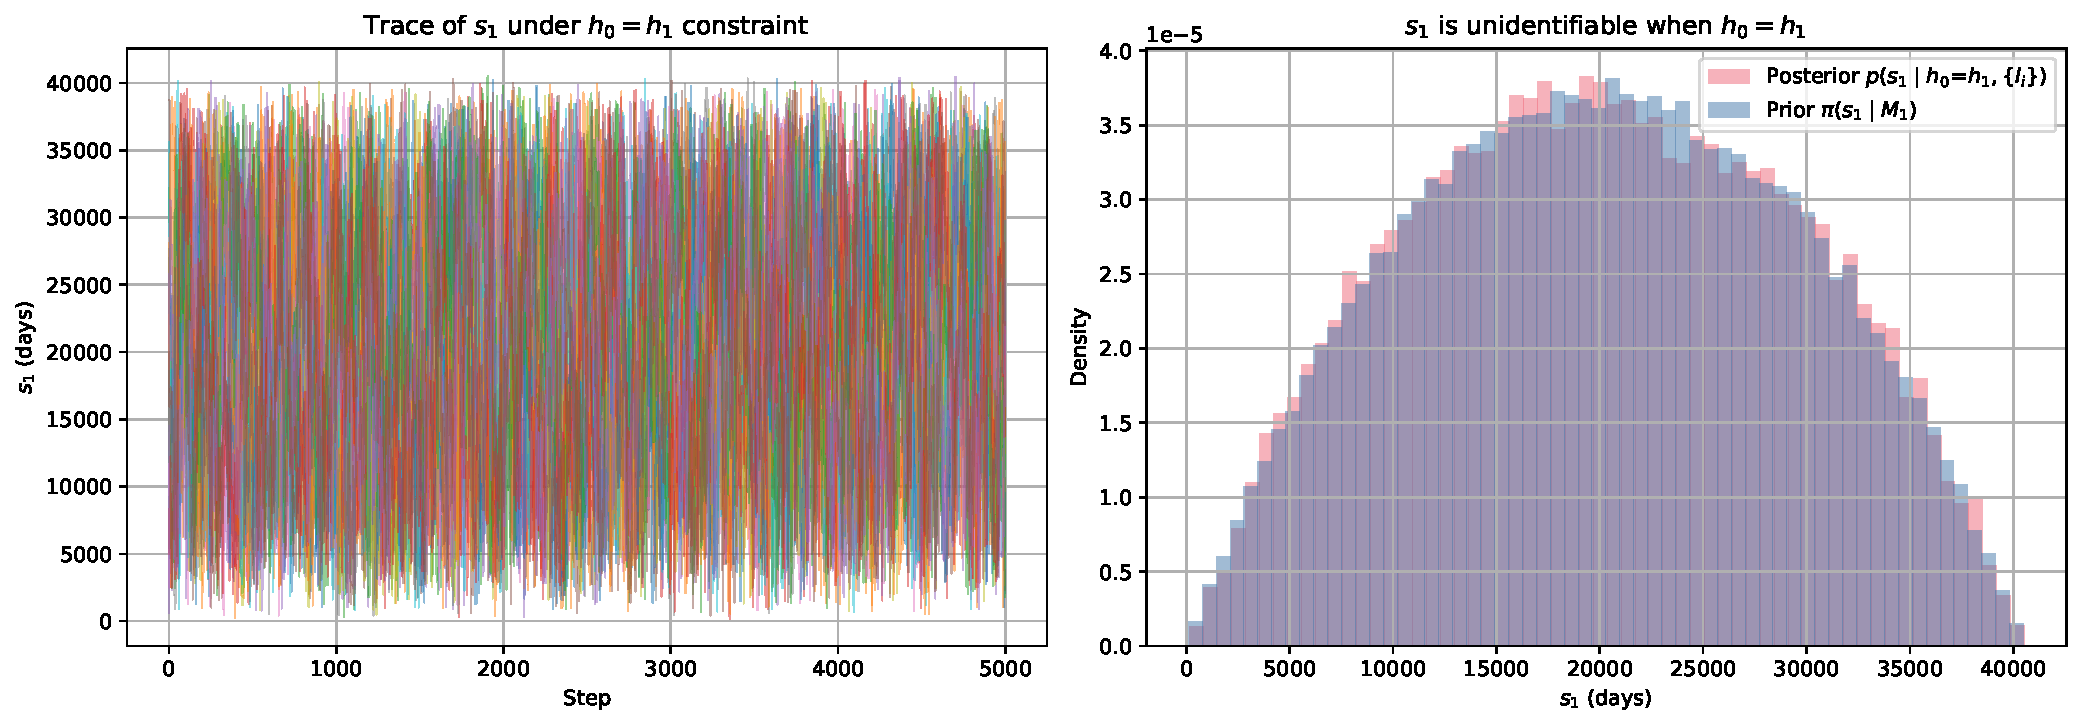
\includegraphics[width=\textwidth]{figs/q4b_savage_dickey.pdf}
  \caption{Illustration of the Savage--Dickey difficulty. When $h_0 = h_1$, the posterior on $s_1$ reverts to the prior, and $\delta = 0$ lies deep in the tail of the unconstrained posterior.}
  \label{fig:q4b}
\end{figure}

\subsection*{(c) Laplace approximation}

The Laplace approximation estimates the evidence by fitting a multivariate Gaussian to the log-posterior at its mode:
\[
  Z_1 \approx (2\pi)^{d/2}\,|\hat{\Sigma}|^{1/2}\,\mathcal{L}(\hat{\theta})\,\pi(\hat{\theta}),
\]
where $d = 3$, $\hat{\theta}$ is the MAP estimate, and $\hat{\Sigma}$ is the inverse of the negative Hessian of the log-posterior at $\hat{\theta}$.

The difficulty is that the $M_1$ log-likelihood contains a hard step function at $s_1$: an event at time $y_i$ contributes $\log h_0$ if $y_i < s_1$ and $\log h_1$ otherwise.
The log-likelihood is therefore piecewise linear in $s_1$ between adjacent event times, with discontinuous jumps whenever $s_1$ crosses an event time.
The Hessian $\partial^2 \log P / \partial s_1^2$ is zero almost everywhere with delta-function singularities at each event time --- it is not well defined.
The Gaussian approximation is therefore invalid: the posterior is not smooth in $s_1$, and the Laplace approximation breaks down.

\subsection*{(d) Nested sampling for $M_1$ evidence}

We used \texttt{dynesty}'s static nested sampler with 1000 live points and a stopping criterion of $\Delta \log Z < 0.01$.
The prior transform maps from the unit cube to the physical parameter space via the inverse CDFs of the $\Gamma(1, 200)$ priors for $h_0, h_1$ and the $\text{Beta}(2, 2)$ prior (scaled to $[0, L]$) for $s_1$.
The log-likelihood is the same piecewise-constant Poisson process expression used in the MCMC --- \texttt{dynesty} requires no gradients, so the discontinuity in $s_1$ poses no difficulty.
Multi-ellipsoidal decomposition was used for bounding the live-point distribution.

The results are:
\begin{align*}
  \log Z_1 &= -1187.54 \pm 0.12, \\
  \log Z_0 &= -1217.09 \quad\text{(analytic, from Q3a)}, \\
  \log B_{10} &= \log(Z_1/Z_0) = 29.56, \quad B_{10} \approx 6.85 \times 10^{12}.
\end{align*}
The prior odds are $\pi(M_1)/\pi(M_0) = \lambda = 3$ (from the truncated Poisson prior on $k$), giving
\[
  \text{Posterior odds} = B_{10} \times \frac{\pi(M_1)}{\pi(M_0)} \approx 2.05 \times 10^{13}.
\]
The data overwhelmingly favour $M_1$ over $M_0$.

%----------------------------------------------------------------------
\section*{Question 5 --- The $k$ change-point models, $M_k$}
%----------------------------------------------------------------------

\subsection*{(b) RJMCMC trace and posterior on $k$}

The reversible jump MCMC sampler was run for $10^5$ iterations.
Figure~\ref{fig:q5b} shows the trace plot for the model index $k$ and the posterior distribution on $k$.
The trace plot confirms that the chain explores the model space thoroughly, visiting a wide range of $k$ values with rapid mixing.

The maximum \emph{a posteriori} (MAP) number of change points is $\mathbf{k = 3}$, with posterior probability $P(k=3 \mid \{I_i\}) = 0.279$.
The top five values are $k = 3$ (0.279), $k = 2$ (0.261), $k = 4$ (0.218), $k = 5$ (0.104), and $k = 1$ (0.087).

\begin{figure}[ht]
  \centering
  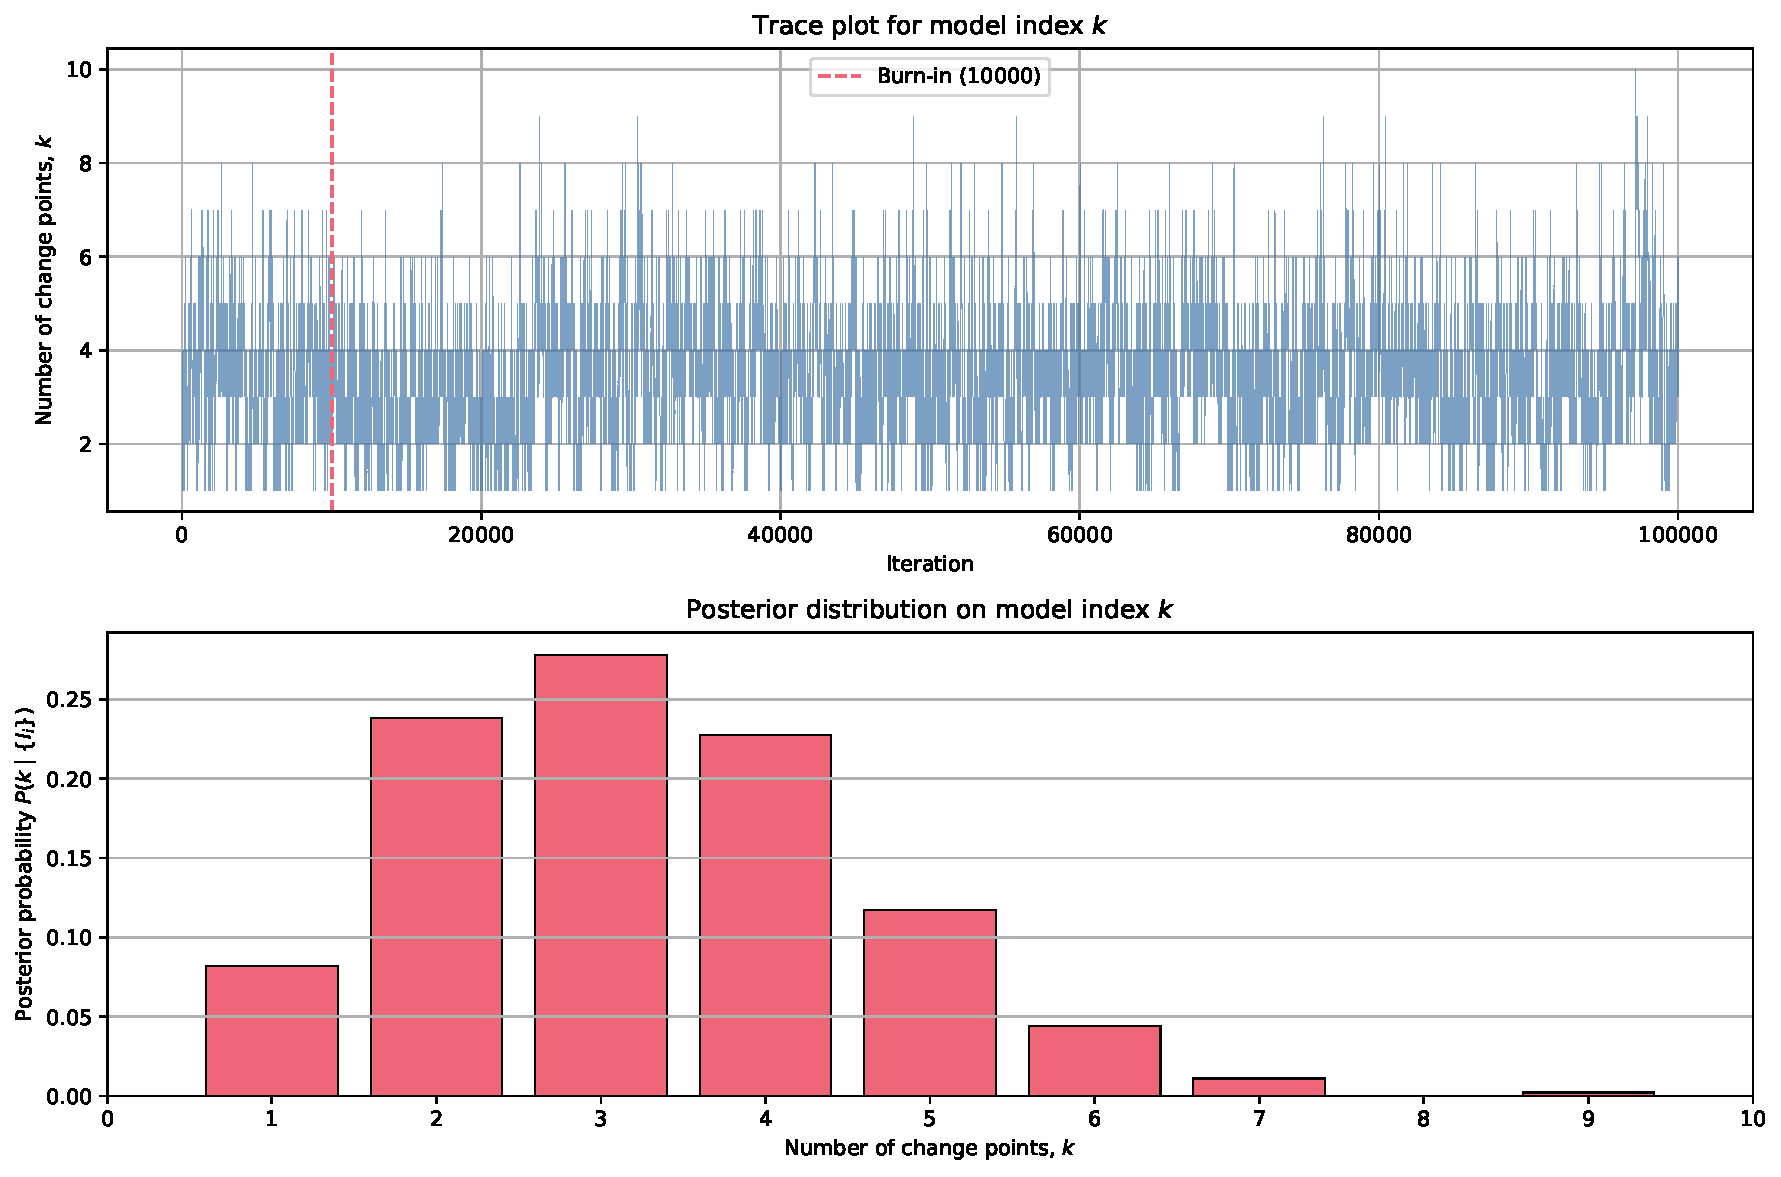
\includegraphics[width=\textwidth]{figs/q5b_rjmcmc_k.pdf}
  \caption{Top: trace plot for the model index $k$. Bottom: posterior distribution on $k$.}
  \label{fig:q5b}
\end{figure}

\subsection*{(c) Inferred rate with uncertainty}

Figure~\ref{fig:q5c} shows the model-averaged inferred accident rate $x(t)$ with 50\% and 90\% credible regions.

\textbf{Calculating the uncertainty regions.}
For each post-burn-in RJMCMC sample, the state encodes a complete step-function rate $x(t)$ with a particular number of change points $k$, change-point positions, and segment rates.
Each sample's rate function was evaluated on a dense grid of 1000 time points spanning the observation period.
This produces, at each grid point, an ensemble of rate values drawn from the full model-averaged posterior --- samples with different $k$ contribute naturally since the RJMCMC chain explores the joint space of all models.
The 50\% credible region is the interval between the 25th and 75th percentiles of this ensemble at each time point, and the 90\% region spans the 5th to 95th percentiles.
The median is the pointwise 50th percentile.
These are pointwise credible intervals, not simultaneous bands.

\begin{figure}[ht]
  \centering
  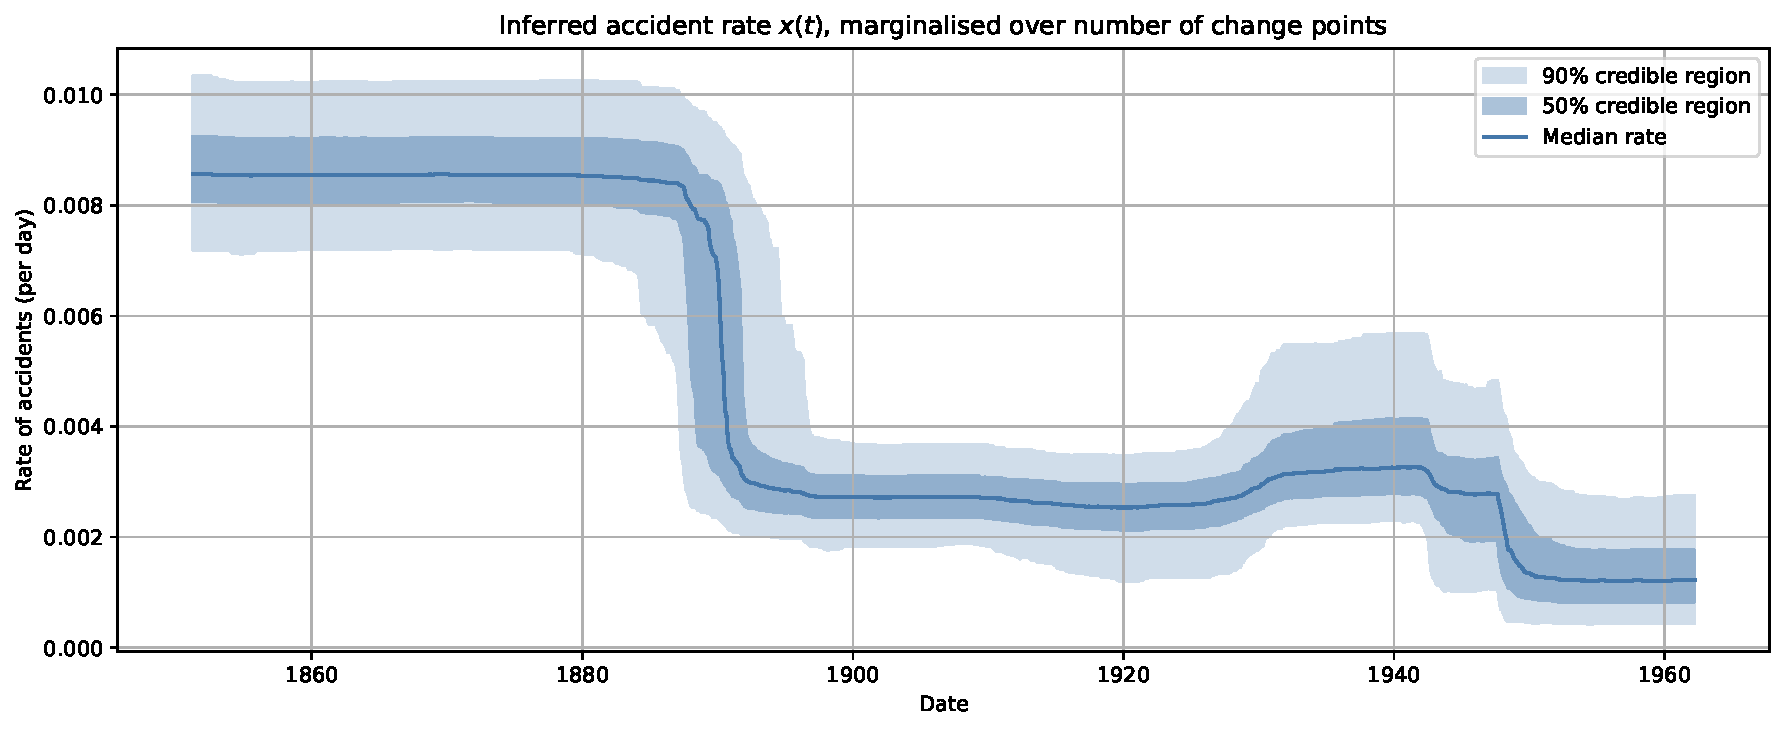
\includegraphics[width=\textwidth]{figs/q5c_inferred_rate.pdf}
  \caption{Inferred accident rate $x(t)$ marginalised over the number of change points, with 50\% and 90\% pointwise credible regions.}
  \label{fig:q5c}
\end{figure}

%----------------------------------------------------------------------
\section*{Declaration of use of autogeneration tools}
%----------------------------------------------------------------------

Claude Code (Anthropic) was used as a coding assistant throughout this coursework for: code scaffolding, debugging, plotting, and drafting written explanations. All outputs were reviewed, verified, and edited by the author. The mathematical derivations and scientific interpretations reflect the author's own understanding.

\end{document}
